\documentclass[a4paper]{report}
\pagestyle{headings}
\usepackage{hyperref}
\usepackage{listings}
\usepackage{graphicx}
\lstset{language=bash}
\lstset{numbers=right}
\lstset{breaklines}
\title{Lab Report for Object-oriented Programming course \newline
 Lab 1: Reversi Game}
\author{Wang, Chen \\ 16307110064 \\ School of Software\\ Fudan University}
\date{\today}
\bibliographystyle{plain}
\begin{document}
\maketitle

\tableofcontents

\chapter{Background Knowledge \& Concepts Required for This Lab}
\section{Reversi Game}
Reversi is a strategy board game for two players, played on an 8 by 8 uncheckered board. There are sixty-four identical game pieces called disks (often spelled "discs"), which are light on one side and dark on the other. Players take turns placing disks on the board with their assigned color facing up. During a play, any disks of the opponent's color that are in a straight line and bounded by the disk just placed and another disk of the current player's color are turned over to the current player's color. 
\par
The object of the game is to have the majority of disks turned to display your color when the last playable empty square is filled. 
\par
Reversi was most recently marketed by Mattel under the trademark Othello. 

\subsection{Original Version of History}
The game Reversi was invented in 1883 by either of two Englishmen (each claiming the other to be a fraud), Lewis Waterman or John W. Mollett (or perhaps earlier by someone else entirely), and gained considerable popularity in England at the end of the nineteenth century. The game's first reliable mention is in the 21 August 1886 edition of The Saturday Review. Later mention includes an 1895 article in The New York Times: "Reversi is something like Go Bang, and is played with 64 pieces." In 1893, the German games publisher Ravensburger started producing the game as one of its first titles. Two 18th-century continental European books dealing with a game that may or may not be Reversi are mentioned on page fourteen of the Spring 1989 Othello Quarterly, and there has been speculation, so far without documentation, that the game has older origins.

\subsection{Modern Version of History}
The modern version of the game — the most regularly used rule-set, and the one used in international tournaments — is marketed and recognized as Othello. It was patented in Japan in 1971 by Goro Hasegawa (autonym: Satoshi Hasegawa), then a 38-year-old salesman.
\par
There is one difference from the original game: 
\begin{enumerate}
\item The first four pieces go in the center, but in a standard diagonal pattern, rather than being placed by players.
\end{enumerate}
According to Ben Seeley, another difference of Reversi from Othello is that in the first one the game ends as soon as either player cannot make a move, while in the latter the player without a move simply passes.
\par
Hasegawa established the Japan Othello Association on March 1973, and held the first national Othello championship on April 4, 1973 in Japan. The Japanese game company Tsukuda Original launched Othello in late April, 1973 in Japan under Hasegawa’s license, which led to an immediate commercial success.
\par
The name was selected by Hasegawa as a reference to the Shakespearean play Othello, the Moor of Venice, referring to the conflict between the Moor Othello and Iago, and more controversially, to the unfolding drama between Othello, who is black, and Desdemona, who is white. The green color of the board is inspired by the image of the general Othello, valiantly leading his battle in a green field. It can also be likened to a jealousy competition (jealousy being the central theme in Shakespeare's play, which popularized the term "green-eyed monster"), since players engulf the pieces of the opponent, thereby turning them to their possession. 
\par
Othello was first launched in the U.S. in 1975 by Gabriel Industries and it also enjoyed commercial success there. Reportedly, Othello game sales have exceeded \$600 million and more than 40 million classic games have been sold in over 100 different countries. 
\par
Hasegawa also wrote How to Othello (Osero No Uchikata) in Japan in 1974, which was later translated into English and published in the U.S. in 1977 as How to Win at Othello.
\par
Kabushiki Kaisha Othello, which is owned by Hasegawa, registered the trademark "OTHELLO" for board games in Japan and Tsukuda Original registered the mark in the rest of the world. All intellectual property regarding Othello outside Japan is now owned by MegaHouse, a Japanese toy company that acquired PalBox, the successor to Tsukuda Original.

\subsection{Rules}
Each of the disks' two sides corresponds to one player; they are referred to here as light and dark after the sides of Othello pieces, but any counters with distinctive faces are suitable. The game may for example be played with a chessboard and Scrabble pieces, with one player letters and the other backs. 
\par
The historical version of Reversi starts with an empty board, and the first two moves by each player are in the four central squares of the board. The players place their disks alternately with their color facing up and no captures are made. A player may choose to not play both pieces on the same diagonal, different from the standard Othello opening. It is also possible to play variants of Reversi and Othello wherein the second player's second move may or must flip one of the opposite-colored disks (as variants closest to the normal games). 
\par
For the specific game of Othello (as technically differing from the historical Reversi), the rules state that the game begins with four disks placed in a square in the middle of the grid, two facing white side up, two pieces with the dark side up, with same-colored disks on a diagonal with each other. Convention has initial board position such that the disks with dark side up are to the north-east and south-west (from both players' perspectives), though this is only marginally meaningful to play (where opening memorization is an issue, some players may benefit from consistency on this). If the disks with dark side up are to the north-west and south-east, the board may be rotated by 90 degrees clockwise or counterclockwise. The dark player moves first. 
\par
In common practice over the internet, opponents agree upon a time-control of, typically, from one to thirty minutes per game per player. Standard time control in the World Championship is thirty minutes, and this or something close to it is common in over-the-board (as opposed to internet) tournament play generally. In time-defaulted games, where disk differential is used for tie-breaks in tournaments or for rating purposes, one common over-the-board procedure for the winner of defaulted contests to complete both sides' moves with the greater of the result thereby or one disk difference in the winner's favor being the recorded score. Games in which both players have the same number of disks their color at the end (almost always with a full-board 32–32 score) are not very common, but also not rare, and these are designated as 'ties' and scored as half of a win for each player in tournaments. The term 'draw' for such may also be heard, but is somewhat frowned upon. 
\par
What are generally referred to as transcript sheets are generally in use in tournament over-the-board play, with both players obligated to record their game's moves by placing the number of each move in an 8 by 8 grid. This both enables players to look up past games of note and tournament directors and players to resolve disputes (according to whatever specific rules are in place) where claims that an illegal move, flip or other anomaly are voiced. An alternative recording method not requiring a grid is also in use, where positions on a board are labeled left to right by letters a through h and top to bottom (far-to-near) by digits 1 through 8 (Note that this is the opposite of the chess standard, with numerals running upward away from the side (White) that has a through h left to right, and also that the perspective may be that of either player (with no fixed standard)), so that the very first move of a game may be (based upon standard starting setup) d3, c4, f5 or e6. This alternate notational scheme is used primarily in verbal discussions or where a linear representation is desirable in print, but may also be permissible as during-game transcription by either or both players. 
\par
Tournament play using ordinary sets rather than a computer interface—where this can not be an issue—have various ways of handling illegal moves and over- or underflipping (flips that should not be made but are or should be but are not). For example, permitting either player (perpetrator or its opponent) to make a correction going back some fixed number of moves (after which no remedy is available) is one procedure that has been used. 
\par
Significant variants of the game, such as where the starting position differs from standard or the objective is to have the fewest pieces one's color at the end, are sometimes—but rarely—played. 
\subsection{Computer opponents and research}

Good Othello computer programs play very strong against human opponents. This is mostly due to difficulties in human look-ahead peculiar to Othello: The interchangeability of the disks and therefore apparent strategic meaninglessness (as opposed to chess pieces for example) makes an evaluation of different moves much harder. This can be demonstrated with blindfold games, as the memorization of the board demands much more dedication from the players than in blindfold chess. Also the game has been particularly attractive to programmers. Therefore, the best Othello computer programs have easily defeated the best humans since 1980, when the program The Moor beat the reigning world champion. In 1997, Logistello defeated the human champion Takeshi Murakami with a score of 6-0. 
\par
Analysts have estimated the number of legal positions in Othello is at most $10^28$, and it has a game-tree complexity of approximately $10^58$. Mathematically, Othello still remains unsolved. Experts have not absolutely resolved what the outcome of a game will be where both sides use perfect play. However, analysis of thousands of high-quality games (most of them computer-generated) appears to lead to a reliable conclusion (pending actual proof if true) that, on the standard 8 by 8 board, perfect play on both sides results in a draw. When generalizing the game to play on an n by n board, the problem of determining if the first player has a winning move in a given position is PSPACE-complete. On 4 by 4 and 6 by 6 boards under perfect play, the second player wins. The first of these proofs is relatively trivial, and the second dates to around 1990. 

\section{Object-oriented Programming}
Object-oriented programming (OOP) is a programming paradigm based on the concept of "objects", which can contain data, in the form of fields (often known as attributes), and code, in the form of procedures (often known as methods). A feature of objects is an object's procedures that can access and often modify the data fields of the object with which they are associated (objects have a notion of "this" or "self"). In OOP, computer programs are designed by making them out of objects that interact with one another.[1][2] OOP languages are diverse, but the most popular ones are class-based, meaning that objects are instances of classes, which also determine their types. 
\par
Many of the most widely used programming languages (such as C++, Object Pascal, Java, Python, etc.) are multi-paradigm and they support object-oriented programming to a greater or lesser degree, typically in combination with imperative, procedural programming. Significant object-oriented languages include Java, C++, C\#, Python, PHP, JavaScript, Ruby, Perl, Object Pascal, Objective-C, Dart, Swift, Scala, Common Lisp, and Smalltalk. 
\subsection{Features of Object-oriented Programming}
Object-oriented programming uses objects, but not all of the associated techniques and structures are supported directly in languages that claim to support OOP. The features listed below are common among languages considered to be strongly class- and object-oriented (or multi-paradigm with OOP support), with notable exceptions mentioned.
\par
In the subsections below, three most important concepts of object-oriented programming is described.

\subsection{Inheritance}
In object-oriented programming, inheritance is the mechanism of basing an object or class upon another object (prototype-based inheritance) or class (class-based inheritance), retaining similar implementation. Also defined as deriving new classes (sub classes) from existing ones (super class or base class) and forming them into a hierarchy of classes. In most class-based object-oriented languages, an object created through inheritance (a "child object") acquires all the properties and behaviors of the parent object (except: constructors, destructor, overloaded operators and friend functions of the base class). Inheritance allows programmers to create classes that are built upon existing classes, to specify a new implementation while maintaining the same behaviors (realizing an interface), to reuse code and to independently extend original software via public classes and interfaces. The relationships of objects or classes through inheritance give rise to a directed graph. Inheritance was invented in 1969 for Simula.

\subsection{Polymorphism}
In programming languages and type theory, polymorphism is the provision of a single interface to entities of different types or the use of a single symbol to represent multiple different types.
\begin{enumerate}
\item Ad hoc polymorphism: defines a common interface for an arbitrary set of individually specified types.
\item Parametric polymorphism: when one or more types are not specified by name but by abstract symbols that can represent any type.
\item Subtyping (also called subtype polymorphism or inclusion polymorphism): when a name denotes instances of many different classes related by some common superclass.
\end{enumerate}
\par
In C++ and Java, parametric polymorphism is commonly used.
\subsection{Encapsulation}
In object oriented programming languages, encapsulation is used to refer to one of two related but distinct notions, and sometimes to the combination thereof: 
\begin{enumerate}
\item A language mechanism for restricting direct access to some of the object's components.
\item A language construct that facilitates the bundling of data with the methods (or other functions) operating on that data.
\end{enumerate}
Some programming language researchers and academics use the first meaning alone or in combination with the second as a distinguishing feature of object-oriented programming, while some programming languages that provide lexical closures view encapsulation as a feature of the language orthogonal to object orientation. 
The second definition is motivated by the fact that in many of the OOP languages hiding of components is not automatic or can be overridden; thus, information hiding is defined as a separate notion by those who prefer the second definition. 
The features of encapsulation are supported using classes in most object-oriented programming languages, although other alternatives also exist. 

\chapter{Specifications of This Lab}
\section{Regulations in the game}
Each piece in reversi consists of black and white, one side white, one side black. In each move, the piece of the player's side is placed on a vacant place on the board, if the player has its piece in any of the eight directions in horizontal, vertical or diagonal directions and the opponent is sandwiched in the middle, then of all the opponents' sandwiched pieces will be flipped; and you can only play where you can flip the pieces. If a side has at least one legal move to make, he must play without waiver. When the board is full or both sides have no pieces to play, the game is over and the winner is counted by the number of pieces. Before the board is full, if one side's pieces have been eaten by the other side, the game is over and the side that ate up the opponent's pieces wins. 
\par
The game is a complex, strategic game in which scores change dramatically and take a long time to think about. We are only trying to implement a simplified version of the game, in which a person and a computer play black and white, and the computer plays chess according to a predetermined strategy. The detailed regulation of the both sides is specified in the  documentation of the lab requirement document.
\par
The termination conditions of the game in this lab is in consistent with the reversi game. The four conditions where the game terminates are listed below:

\begin{enumerate}
\item the board is full; In the first three cases, the number of pieces is used to calculate the winner. The fourth case decides the other side wins.
\item one party's pieces have been eaten up by the other party; 
\item neither player has a checkerboard to drop;
\item one party falls in an illegal position.
\end{enumerate}
In the first three cases, the number of pieces is used to decide the winner. The fourth case decides the other side wins.
\section{Guidelines for computer side piece placing}
For each possible position, try to calculate the "score" (the number of opponents that can be reversed) for that position, and the higher the score, the better the position. The program should calculate the score for each possible position and select the position with the greatest number of flips. 
\par
Note that there may be two or more places with the same score. In this case, select the place with the samller row character. If two places have the same score and are in the same row, select the place with smaller column numbers. By following the direction of the direction tuple, the program should iterate over the score value and test if it is the highest score value.

\section{Other specifications of the programming}
Below are some other specifications that are required to meet in this lab.
\par
The board should be output to the terminal and the user needs to input the letters representing the position of the piece to be placed. In each turn, the computer should place its piece automatically according to the regulations stated above and the program should ask the user to input his intention. If the user has an invalid input or the game meets other termination conditions, the program should decide the winner, display the corresponding information on the screen and write the log.
\par
As required, the log file is \emph{reversi.csv} under the the package folder of the project. Considering more independence of the system, the line separater of the file is set according to the system and the file encoding is \emph{UTF-8}.
\par
Furthermore, the Javadoc of this project is well-available both in the source code and in the compiled \emph{HTML} files in the \emph{javadoc} folder.

\chapter{Structure and  the OO Ideas Adopted}
\section{Objected-oriented ideas adopted in the implementation}
\subsection{Interfaces}
In my version of implementation, an interface \emph{Playable} is designed to characterize the roles that can play the game. For example, in the current implementation, a \emph{Computer} class and a \emph{Person} class are two classes that implement this interface. This interface makes the unified place piece method available no matter a person or a computer is playing the game. Furthermore, it may function more in the future if the strategy is changed so that there is not one person to one computer playing the game. Any member interacting in the game can implement the \emph{Playable} interface.
\subsection{Abstract classes}
In my version of implementation, an abstract class \emph{Piece} is designed to characterize the pieces that can be placed on the board. For example, in the current implementation, a \emph{BlackPiece} class and a \emph{WhitePiece} concrete class are two classes that extends this abstract class. This abstract class makes the unified piece queries or place methods available no matter a black piece or a white piece is being placed. Furthermore, it may function more in the future if the strategy is changed so that there is two colors of the pieces are to be placed. Any kind of piece to be placed on the board can extend the \emph{Piece} abstract class.
\subsection{Inheritance}
The character of inheritance is widely adopted among the classes in the classes. As stated above, the classes like \emph{Piece} and the player classes all have inheritance relationships. By using inheritance, the methods of parent classes can be well-reused by the child classes and the method names are unified. Furthermore, inheritance makes polymorphism available.
\subsection{Polymorphism}
Thanks to the interfaces, the abstract classes and the inheritance relationships defined above, polymorphism is widely appeared in the program. For example, the following code snippet is an example of polymorphism displayed in this program, the code is in the \emph{placeable} method in the \emph{Computer} class:
\begin{lstlisting}[language=java]
if (!piece.placeable(board, false)) {
    if (piece.placeable(board, true))
        System.out.print(board.computerPieceName + " player has no valid move. ");
    return false;
}
\end{lstlisting}
In this code, the variable \emph{piece} is declared with the abstract class \emph{Piece}, and the actual type of this variable cannot be determined until the runtime. The runtime type of this variable is according to the color of the piece that the user selected. In the code snippet above, the method is called directly via the abstract method in the parent class and the corresponding concrete method will be called at runtime.
\section{UML Diagram for the structure of the project}
\begin{figure}
  \centering
  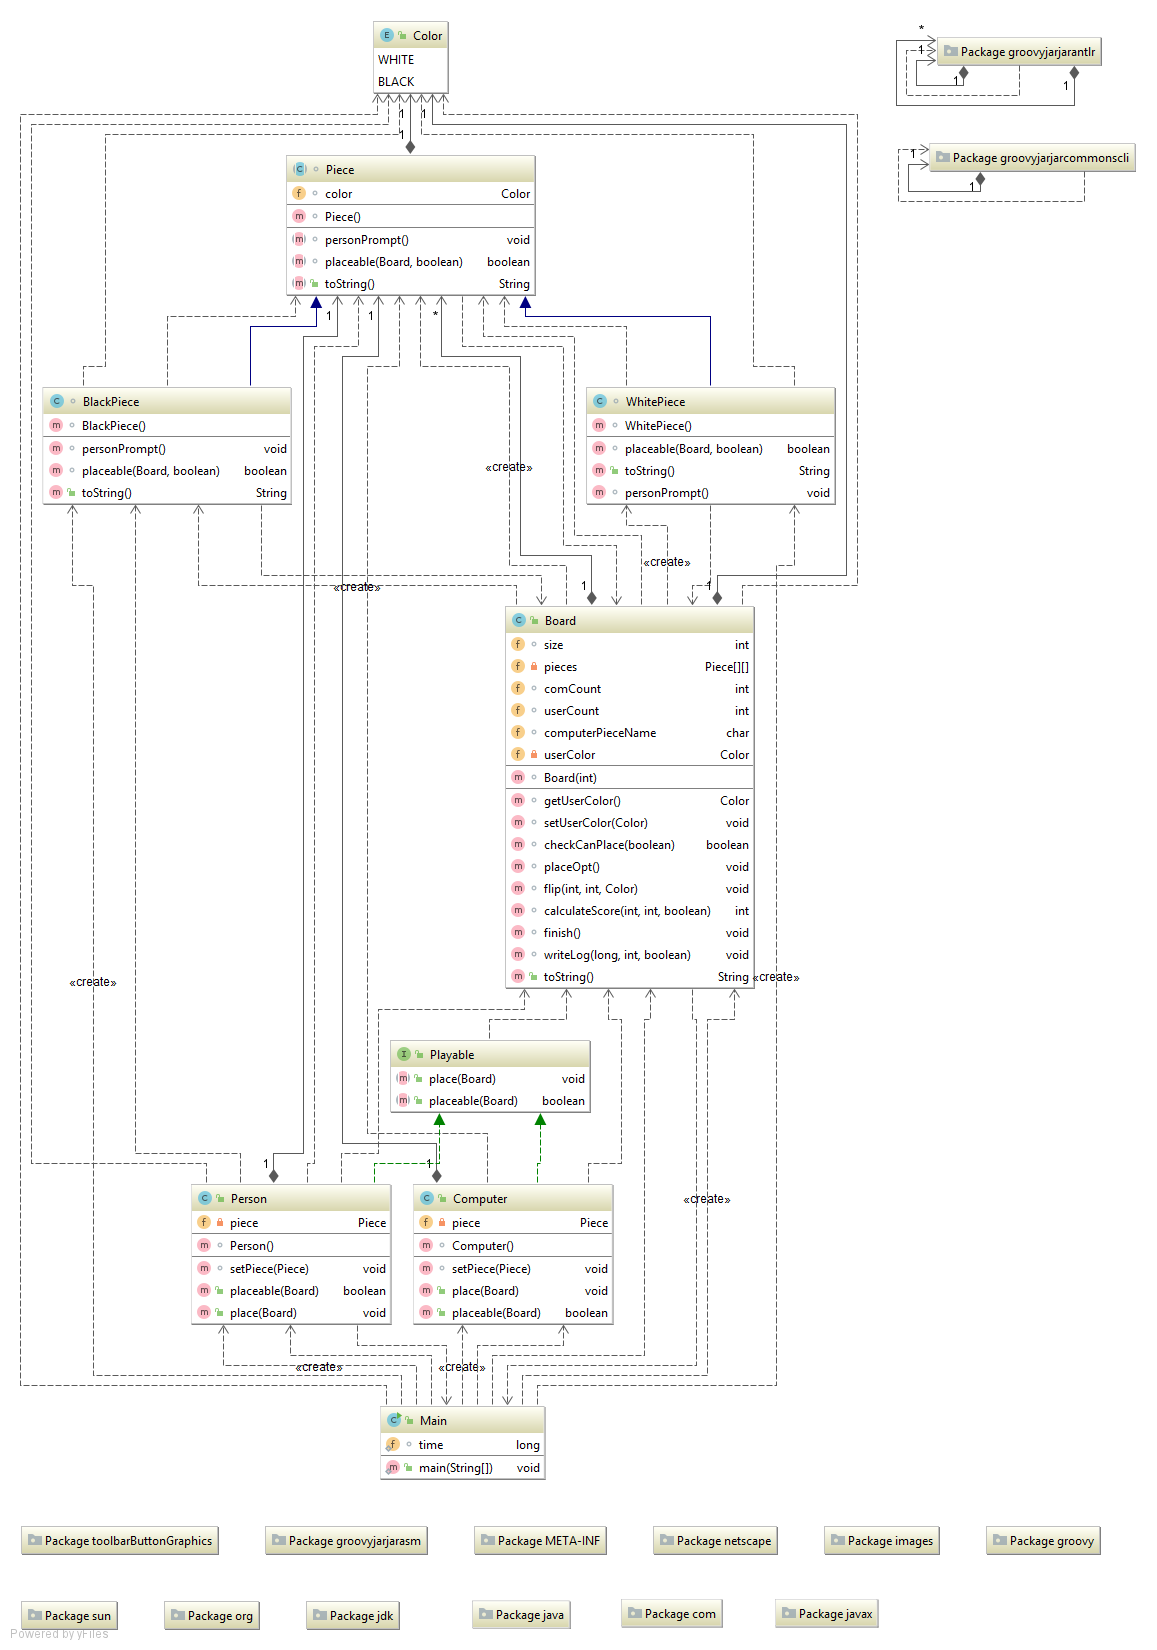
\includegraphics[width=14cm]{Top-LevelPackage.png}
  \caption{UML diagram of top-level package}\label{1}
\end{figure}

\chapter{Running Result of My Implementation}






\begin{thebibliography}{A}

\bibitem{1}
Wikipedia contributors. (2018, December 24). Version control. In \emph{Wikipedia, The Free Encyclopedia}. Retrieved 06:12, March 10, 2019, from \url{https://en.wikipedia.org/w/index.php?title=Version_control&oldid=875227317}

\bibitem{2}
Wikipedia contributors. (2019, March 10). Systems development life cycle. In \emph{Wikipedia, The Free Encyclopedia}. Retrieved 06:13, March 10, 2019, from \url{https://en.wikipedia.org/w/index.php?title=Systems_development_life_cycle&oldid=887015682}

\bibitem{3}
Stolen, L. H. (1999). Distributed control system. \emph{international telecommunications energy conference.}

\bibitem{4}
Murayama, T. (1991). Distributed Control System. \emph{international conference on advanced robotics robots in unstructured environments}.

\bibitem{5}
Wikipedia contributors. (2019, March 6). Distributed control system. In \emph{Wikipedia, The Free Encyclopedia}. Retrieved 06:18, March 10, 2019, from \url{https://en.wikipedia.org/w/index.php?title=Distributed_control_system&oldid=886468871}

\end{thebibliography}
\end{document} 